% warning: use pdflatex to compile!
\documentclass[pdftex,12pt,a4paper]{report}
\usepackage{dbstmpl}
\usepackage{subfigure}
\usepackage{graphicx}
\usepackage{url}
\usepackage{tikz}
\usetikzlibrary{arrows,shapes,positioning}
\usepackage{algorithm}
\usepackage{algpseudocode}
\algnewcommand\algorithmicforeach{\textbf{for each}}
\algdef{S}[FOR]{ForEach}[1]{\algorithmicforeach\ #1\ \algorithmicdo}
\usepackage{tabularx}

\global\arbeit{Bachelorarbeit}
\global\titel{Efficient Event Classification through Constrained Subgraph Mining}
\global\bearbeiter{Simon Lackerbauer}
\global\betreuer{Martin Ringsquandl}
\global\aufgabensteller{Prof. Dr. Peer Kr"oger}
\global\abgabetermin{16. Februar 2018}
\global\ort{M"unchen}
\global\fach{Informatik}

\begin{document}

\deckblatt
\erklaerung

\begin{abstract}
With this work, I consider the problem of discovering patterns in error log data predicting common failure modes within a near fully-automated assembly line. I present a novel approach of encoding error log events in a graph structure and leverage a constraint based mining method to efficiently discover and score sophisticated patterns in these data, using a self implemented version of the pattern-growth algorithm \textit{gSpan}. As the algorithm as implemented does not scale quite as well as many traditional sequential pattern mining approaches, outside expert knowledge should be used to keep the input data to a manageable size and help with graph construction.
\end{abstract}

\tableofcontents

\chapter{Introduction}
The ability to analyze log files is a crucial part in the work of systems administrators and software developers. Developers often enough outright provoke the generation of detailed logs while debugging a piece of software, while system and network operators are routinely pulled from their efforts to fine tune services by incessant alerts from their monitoring systems.

Indeed, transaction log files, a common subgroup of the more general event logs, have been used to diagnose errors in the workings of data processing systems nearly since their inception, and dedicated research efforts into the analysis of transaction log files can be traced back until at least the mid-1960s.\cite{Peters1993-fw}

With the decline of monolithic service architectures, and the recent rise of complex systems of interdependent microservices,\cite{Dragoni2016-fh} the accurate reading of log files and recognition of the patterns within has become more important than ever. Nowadays, a plethora of log file management and search tools exist as both open source and commercially licensed tooling.\cite{noauthor_undated-bv}\cite{noauthor_undated-zu}\cite{noauthor_undated-vl}\cite{noauthor_undated-xi} More sophisticated log file analysis that goes beyond simple exploratory data analysis and simple monitoring and alerting systems is, however, not usually the focus of these tools.

But not only modern microservice architectures need powerful log file analysis tools to understand where bottlenecks and emergent properties of the architecture might stem from. That's why, with this bachelor's thesis, I want to leverage these techniques with a slightly more traditional, yet similarly highly modularized, architecture in mind: an automated production line.

Modern automated production lines usually consist of highly sophisticated robotic modules that assemble each produced unit with an efficiency and consistency that would be virtually impossible for human workers to achieve. However, at the same time, such automated systems are less tolerant of errors accumulating along the way and might stop working for relatively mundane reasons like a part being slightly out of position on the assembly line. Unlike a human worker, a specialized robot cannot solve most of these problems by itself. Depending on the problems encountered, the amount of time and (human) effort needed to deal with them can drive up the cost of running the line enormously, maybe even up to the point of operating at a loss.

If problems like these crop up consistently, it is only natural to assume a common cause between propagated failures along the assembly line\cite{Ringsquandl2016-en} and it can be assumed that, after identifying such causes early on and mitigating them, propagation of failures might be reduced or entirely averted. The production line analyzed in this thesis had the goal to optimize their efficiency as well.

Thus, the aim of this thesis will be to work on this problem using a graph mining based approach, starting with an overview of the literature (chapter \ref{chapter:related_work}) and the theoretical basis of graph mining (chapter \ref{chapter:theoretical_basis}), reflecting on how to extract a graph data structure from the data available as a log table (chapter \ref{section:data_set_splicing}), how best to mine the resulting graph or graphs for patterns (chapter \ref{section:gspan}), and eventually how to assess the resulting patterns (chapter \ref{subsection:evaluation}).

\chapter{Related work}
\label{chapter:related_work}
Leveraging a graph mining based approach for mining log data constitutes a relatively novel use for most of the algorithms implemented in this work. Graph mining as a concept, has, up to this point, been mostly used on data that naturally lend themselves to a graph or network based data structure, such as social networks, modeling human relationship networks in general, chemical component analysis or link networks.\cite{Washio2003-fc}\cite{Han2007-qx} Meanwhile, mostly sequential pattern mining approaches have been leveraged against access or error log based data, such as the \textit{basket data} collected by most large retailers nowadays\cite{Agrawal1993-nc} or \textit{web access logs}\cite{Pei2000-rz}. The \textit{gSpan} algorithm was originally tested on synthetic graph data as well as for mining chemical compound data.\cite{Yan2002-sj}

Most of the above mentioned naturally occurring graph data don't include time as a feature having measurable impact on the depicted relations. Chemical compounds may change and degrade over time, but their graph representations usually portray their idealized form. Social networks have also been of interest as dynamic processes themselves,\cite{Kossinets2006-rw} but these analyses tend to focus on snapshots of the full network after longer periods of time, whereas the data set examined in this work is a classical time series, with each row explicitly time stamped down to the second.

\section{Sequential pattern mining}
Sequential pattern analysis is a staple approach in time series mining. The term was first introduced and defined by Agrawal and Srikant\cite{Agrawal1994-ca} as follows: 
\begin{quotation}
	[G]iven a sequence database where each sequence is a list of transactions ordered by transaction time and each transaction consists of a set of items, find all sequential patterns with a user-specified minimum support, where the support is the number of data sequences that contain the pattern.
\end{quotation}

More formally, let $I = \{i_0, i_1, ..., i_n\}$ be a set of all items. Then a $k$-itemset $I^*$, which consists of $k$ items from $I$, is said to be \textit{frequent} if it occurs in a transaction database $D$ no less than $\theta|D|$ times, where $\theta$ is a user-specified \textit{minimum support threshold} (often abbreviated \textit{min\_sup}).

Mining sequential patterns can take the form of a-priori algorithms (see subsection \ref{subsection:apriori}), like Srikant and Agrawal's GSP\cite{Srikant1996-dy} or pattern growth algorithms, like Yan and Han's \textit{gSpan}\cite{Yan2002-sj} used in this work.

\section{Classical graph mining approaches}
The classical graph mining approach often focuses on obtaining general structural information about a network. As an example, the mining of social networks often reveals an overall structure of almost-leaves (e.g. friend- or kinship groups) being connected via so called ''multiplicators`` or ''influencers`` -- nodes with a high degree centrality\cite{Newman2010-ac} that are also interconnected with each other, together acting as the central cluster in a basically star-shaped network, which offers an explanation for the small world problem\cite{Travers1967-cn}.

Meanwhile, for this work, the overall structure of the graph (the dependency network between modules and inputs for the assembly line) is known beforehand, and even formally defined. Analysis of the design of the found substructures -- viz. \textit{what} the pattern symbolizes as opposed to \textit{finding} it in the first place -- is indeed only of interest after most of the work is already done.

\subsection{A-priori based approach}
\label{subsection:apriori}
The A-priori based paradigm to frequent pattern mining is a heuristic that generates a reduced set of patterns through each iteration.\cite{Pei2000-rz} The a-priori principle, on which these approaches are based on, states that \textit{any super-pattern of an infrequent pattern cannot be frequent}.\cite{Han2004-qs} Thus, these algorithms first generate a set of all frequent 1-element sequences. From that, they generate new candidate sequences in a step-wise way. For example, if the patterns \textit{A} and \textit{B} are each frequent according to a specific \textit{min\_sup}, then the pattern \textit{AB} might be frequent as well. These generated patterns are then tested and discarded if and only if they don't reach the given \textit{min\_sup} (cf. algorithm \ref{alg:apriori}, where $T$ is the transaction database and $C_k$ is the candidate set for sequence length k).

\begin{algorithm}
	\caption[APriori($T,min\_sup$)]{APriori($T,min\_sup$)\cite{Agrawal1994-ca}}\label{alg:apriori}
	\begin{algorithmic}[1]
		\State {$L_1 \gets$ \{large 1-itemsets\};}
		\State {$k \gets 2$}
		\While {$L_{k-1} \neq \emptyset$}
		\State {$C_k \gets \{ a \cup \{b\} \mid a \in L_{k-1} \land b \not \in a \} - \{ c \mid \{ s \mid s \subseteq c \land |s| = k-1 \} \nsubseteq L_{k-1} \}$}
		\ForEach {$t \in T$}
		\State {$C_t \gets \{ c \mid c \in C_k \land c \subseteq t \}$}
		\ForEach {$c \in C_t$}
		\State {$count[c] \gets count[c] + 1$}
		\EndFor
		\EndFor
		\State {$L_k \gets \{c|c \in C_k \land count[c] \geq min\_sup\}$}
		\State {$k \gets k+1$}
		\EndWhile \\
		\Return {$\bigcup_k L_k$;}
	\end{algorithmic}
\end{algorithm}

Well-studied a-priori-based algorithms include the already mentioned GSP\cite{Srikant1996-dy}, SPADE\cite{Zaki2001-jy}, or HitSet\cite{Han1999-bj}. As a-priori-based approaches have to search through the input data at least once for every candidate pattern, the best a-priori algorithms achieve runtime efficiencies of $O(n^2)$.

\subsection{Pattern-growth based approach}
In contrast, the pattern-growth approach adopts a divide-and-conquer principle as follows: \textit{sequence databases are recursively projected into a set of smaller projected databases based on the current sequential pattern(s), and sequential patterns are grown in each projected database by exploring only locally frequent fragments}.\cite{Han2004-qs} The \textit{gSpan}-algorithm used in this work is, like its predecessors \textit{FreeSpan} and \textit{PrefixSpan}, such a pattern-growth based approach.

\chapter{Theoretical basis}
\label{chapter:theoretical_basis}
The proposed event classification method mines a graph set $\mathcal{D} = (G_0, ..., G_n)$ for substructures of interest, often called ``patterns'' in the literature. To establish a firm theoretical understanding of what the these structures are, some definitions of graph theory are in order.

\section{Graph}
Traditionally, a graph is represented as a set of vertices $V$ and a set of edges $E$, with a mapping $f : E \rightarrow V \times V$ that defines each edge as a tuple of vertices. In directed graphs, this tuple is ordered. In undirected graphs, it is unordered, so that $\forall v_i, v_j: (v_i, v_j) \in E \rightarrow (v_j, v_i) \in E$. In this work, the vertex set $V$ of a graph $G$ may also be denoted $V(G)$. Likewise, the edge set may be denoted $E(G)$. To encode these structures in software, adjacency matrices and edge lists are commonly deployed. The following example adjacency matrix (table \ref{tab:example_adj_mat}) and visual representation (figure \ref{fig:example_graph}) all encode the same undirected graph $G = \left(\{v_1, v_2, v_3, v_4\}, \{(v_1, v_2), (v_2,v_3), (v_3, v_4), (v_4, v_2)\}\right)$.

\begin{table*}
	\caption{Adjacency matrix for graph $G$}
	\label{tab:example_adj_mat}
	\centering
	\begin{tabular}{l|cccc}
		      & $v_1$ & $v_2$ & $v_3$ & $v_4$ \\ \hline
		$v_1$ &   0   &   1   &   0   &   0    \\
		$v_2$ &   1   &   0   &   1   &   1   \\
		$v_3$ &   0   &   1   &   0   &   1   \\
		$v_4$ &   0   &   1   &   1   &   0
	\end{tabular}
\end{table*}

\begin{figure}
	\centering
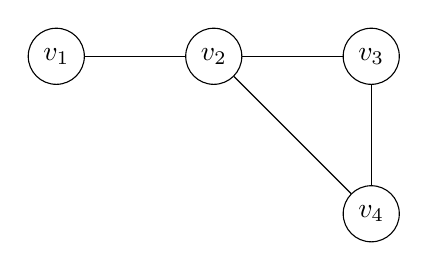
\begin{tikzpicture}[node distance = 2cm]
	\tikzset{VertexStyle/.style = {
			shape=circle,
			draw=black
	}}
	\node[VertexStyle] (1){$v_1$};
	\node[VertexStyle, right of= 1] (2){$v_2$};	
	\node[VertexStyle, right of= 2] (3){$v_3$};
	\node[VertexStyle, below of= 2, right of=2] (4){$v_4$};
	
	\path [-] (1) edge node[above] {} (2);
	\path [-] (2) edge node[above] {} (3);
	\path [-] (3) edge node[left] {} (4);
	\path [-] (2) edge node[left] {} (4);
	\end{tikzpicture}
	\caption[Visual representation of graph $G$]{Visual representation of graph $G$}
	\label{fig:example_graph}
\end{figure}
\section{Subgraph}
Let $G_s$ and $G$ be two graphs, where $G_s = (V_s, E_s)$ and $V_s \subset V(G), E_s \subset E(G)$. Then, if the following holds:
\[ \forall (v_i, v_j) \in E_s \implies v_i, v_j \in V_s, \]
$G_s$ is said to be a subgraph of $G$. Figure \ref{fig:example_subgraph} illustrates an example subgraph of $G$ with three of $G$'s four vertices and two of its four edges. Note that the graphical representation need not be drawn in the same way to depict a subgraph.

\begin{figure}[h]
	\centering
	\begin{tikzpicture}[node distance = 2cm]
	\tikzset{VertexStyle/.style = {
			shape=circle,
			draw=black
	}}
	\node[VertexStyle, right of= 1] (2){$v_2$};	
	\node[VertexStyle, right of= 2, below of=2] (3){$v_3$};
	\node[VertexStyle, right of=3, above of=3] (4){$v_4$};
	

	\path [-] (2) edge node[above] {} (3);
	\path [-] (3) edge node[left] {} (4);
	\end{tikzpicture}
	\caption{Example subgraph $G_s$ of $G$}
	\label{fig:example_subgraph}
\end{figure}


\section{(Sub-)Graph isomorphism}
Two graphs $G$ and $H$ are said to be isomorph when the following holds: let $f: V(G) \rightarrow V(H)$ be a bijection and let vertices $u$ and $v$ of $G$ be adjacent in $G$. Then $G \simeq H$ if and only if $f(u)$ and $f(v)$ are adjacent in $H$. It is currently unknown if the graph isomorphism problem is P or NP.\cite{Fortin1996-la}

The subgraph isomorphism problem is the decision problem of whether, when given two graphs $G$ and $H$, there exists a subgraph in $G$ that is isomorphic to $H$. The subgraph isomorphism problem is known to be NP-complete.\cite{Cook1971-fj}.

\chapter{Methodology}
Especially considering time as both an explicit attribute of nodes and edges, as well as implicitly encoded into the graph structure and as such still present in subsequently mined subgraphs, constitutes an approach to exploring log data through graph mining that has not been examined extensively before.

\section{Disregarded approaches}
Before homing in on analyzing the given data set with \textit{gSpan} and a \textit{Support Vector Machine}, some approaches with lesser quality results were taken. Even though these approaches didn't prove fruitful in the long run, they helped me understand the data set and its underlying structure better and as such are, with their basic premises, included here to give a full account of all measures taken.

\subsection{Shortest path algorithms on a single graph}
\begin{figure}
	\centering
	\noindent\includegraphics[width=\linewidth]{images/fullgraph}
	\caption{Naive single graph encoding all available information}
	\label{fig:fullgraph}
\end{figure}

As the manufacturing process consists of a circuit of interconnected modules, the first approach of translating the given data into a graph form was to build one single large graph with all information available around this first circuit of module nodes, with the intention of later on mining frequent patterns from this single large graph, using algorithms such as Elseidy et al's \textit{GRAMI}\cite{Elseidy2014-fz} or Moussaoui et al's \textit{POSGRAMI}\cite{Moussaoui2016-ng}.

To encode the log error data on top of this framework, the error messages were split into terms (essentially words) and each term made a node. Edges were drawn between all term-nodes in a given message, as well as between all term-nodes and the module-node they occurred in, as well as between all term-nodes and the production-unit-ID-node. This first naive approach of visualizing the available data produced a graph consisting of 523 nodes connected by 2,182 edges (illustrated in figure \ref{fig:fullgraph}). Edges were weighted simply by a count of how often they appeared throughout the whole data set, with some edges only appearing once and a maximum weight of over 10,000 appearances.

This first graph did not, to a first approximation, retain its expected circuit-like appearance, instead clustering heavily around a few modules and production unit IDs that produced the most errors, meaning there were parts in the system vastly more error prone than others.

In a second step, the Dijkstra shortest paths algorithm was used to find all paths between nodes that had a full path length of less than a specific constant, afterwards ordered by path length. For example, a short 4-edge path could connect two modules and the part ID via two error terms, indicating some kind of correlation, much like a sequential pattern analysis could find.

For Dijkstra to work, the naive edge weight for edge $i$ ($w_{i_{naive}}$) had to be transformed from simple counts to a normalized form that would retain comparison operations between edges, but invert path lengths (as the Dijkstra algorithm is used, as its name suggests, to find the \emph{shortest paths}). This was achieved by the following transformation being calculated after graph generation, with~$w_{all}~=~\sum_{j=0}^{n} w_{j_{naive}}$:
\[w_{i_{normalized}} = -\ln \left( \frac{w_{i_{naive}}}{w_{all}} \right) \]

This weight was later penalized further by adding time constraints, so that
\[w_{i_{penalized}} = w_{i_{normalized}} + P(i)\]

where
\[P(i) = \begin{cases}
	\log_{\tilde{\Delta t}} \frac{\Delta t}{C(\Delta t) \cdot \tilde{\Delta t}}, & \text{if }C(\Delta t), \tilde{\Delta t} > 0 \\
	0, & \text{otherwise}
\end{cases}\]

Here, $\Delta t$ is the amount of time between rows being connected by the edge, $C(\Delta t)$ is the amount of connections between these nodes, and $\tilde{\Delta t}$ is the average time differential between rows overall. This ensured penalization for long times between events (indicating that the events weren't correlated), while similarly rewarding events that happened more often in conjunction.

\begin{figure}
	\centering
	\noindent\includegraphics[width=\linewidth]{images/example_pattern}
	\caption{Large example pattern}
	\label{fig:example_patterns}
\end{figure}

\begin{figure}
	\centering
	\noindent\includegraphics[width=\linewidth]{images/small_pattern}
	\caption{Smaller example pattern}
	\label{fig:small_pattern}
\end{figure}

\subsection{Digraph}
Using a directed graph was briefly considered, but did, in some first tests, not lead to noticeably different patterns from the undirected graph. This was almost expected, as graph connections were highly predictable, because of the construction of the graphs similar to dependency graphs. 

If, for example, in one splice, specific terms had a directed edge \textit{towards} a specific module, then this basic structure would obviously be repeated in other slices as well, by virtue of a construction that always pointed terms towards modules. The simple connectedness attribute that is an edge in an undirected graph already served this purpose implicitly when taking into account this background knowledge used during graph construction.

\subsection{Natural language processing}
The idea of combining both techniques of graph mining and a natural language processing unit to make sense of the actual contents of the error logs was briefly entertained as well. Good, easily available NLP software for languages other than English is still quite hard to come by, however. In addition, the analyzed error logs were often very short and technical, and thus didn't lend themselves to an actual content based analysis. Even to native speakers, many of the messages would've been quite cryptic and so it was decided that the processing power that would've been needed for an NLP based approach would be better used elsewhere.

\section{Data set splicing}
\label{section:data_set_splicing}
The investigated data set consisted of about 57,000 messages logged over the course of five consecutive days in October 2016. Available columns were a time stamp (precision: 1s), an unstructured log message in German, the module ID where the message originated and the part ID of the produced item in that run. Messages sometimes included additional partly structured data, like a more detailed report of the location where the error occurred included in the German log message. See table \ref{table:dummy_messages} for an example of the data structure and a part of the synthetic data set used for the testing setup in section \ref{section:synthetic_data_results}.

\begin{table}[]
	\centering
	\caption{Synthetic data set (excerpt)}
	\label{table:dummy_messages}
	\footnotesize 
	\begin{tabular}{l|l|l|l}
		time stamp & log message & module id & part id \\ \hline
		2017-04-05 11:01:05 & Laser "uberhitzt            & Module 1 & 88495775TEST \\
		2017-04-05 11:01:05 & Laser "uberhitzt            & Module 1 & 88495776TEST \\
		2017-04-05 11:01:06 & Teil verkantet             & Module 2 & 88495776TEST \\
		2017-04-05 11:01:06 & Laser "uberhitzt            & Module 1 & 88495776TEST \\
		2017-04-05 11:01:10 & Laser "uberhitzt            & Module 1 & 88495776TEST \\
		2017-04-05 11:01:12 & Auffangbeh"alter leeren     & Module 2 & 88495775TEST \\
		2017-04-05 11:01:17 & Unbekannter Ausnahmefehler & Module 0 & 88495775TEST \\
		2017-04-05 11:01:17 & Auffangbeh"alter leeren     & Module 2 & 88495775TEST \\
		2017-04-05 11:01:19 & Unbekannter Ausnahmefehler & Module 0 & 88495775TEST \\
		2017-04-05 11:05:22 & Laser "uberhitzt            & Module 1 & 88495775TEST \\
		\multicolumn{1}{c}{\vdots} & \multicolumn{1}{c}{\vdots} & \multicolumn{1}{c}{\vdots} & \multicolumn{1}{c}{\vdots}
	\end{tabular}
\end{table}

The data had to be cleaned up slightly prior to a first cursory visual analysis. An, at first glance, large amount of the total message count consisted of (without expert knowledge) seemingly meaningless general error messages consisting of only an error code and no further explanation. These specific messages existed in 4 slightly different formats of about 30 messages with the same time stamp each, with the error code incremented by one with each message. Each instance of these 30 message bursts was replaced with a simple ``general error'' message with the same time stamp. After this preprocessing step, the amount of messages to be considered had roughly halved.

Further, if the module ID and manufacturing unit ID were included in the message in one of several standardized ways, they were extracted and given their own column in the data set to prohibit random integers cropping up in the messages to be mistaken for e.g. a module id.

To generate the graph set to be mined, a week's log data was spliced along 5 minute time frames, producing graphs of the size like exemplified in figure \ref{fig:partial_graph}. Two different modules throwing errors in this specific time window can be easily distinguished. A 3 minute window was briefly considered, but the resulting graphs were, almost surprisingly, much smaller overall, so that the mined patterns weren't open to any meaningful interpretation and were fewer in number as well. Windows smaller than 5 minutes in general mostly led to many more small graphs, so that no long pattern could conceivably ever reach any useful \textit{min\_sup} threshold.

\begin{figure}
	\centering
	\noindent\includegraphics[width=\linewidth]{images/partial_graph}
	\caption{Graph of a 5-minute log data window}
	\label{fig:partial_graph}
\end{figure}

\section{Basic graph construction}
Extracting a basic graph structure from the input is both one of the least computationally intensive steps in the proposed methodology and the most important one. The analyzed data sets don't lend themselves to a natural scheme; background knowledge about the facility had to play an important part in determining the basic structure of the graphs.

As previously mentioned, the constructed graphs heavily relied on known dependencies between error messages, modules and part IDs. Figure \ref{fig:example_slice} illustrates the common connections between the full error message \textit{Z}, its terms \textit{T}, the error logging module \textit{M} and the specific part ID \textit{S}. Error messages could be connected by using common words between them, through, e.g., a further narrowed down standardized localization term, while modules and part ids would be connected to all error messages and their terms produced with their involvement.

\begin{figure}
	\centering
	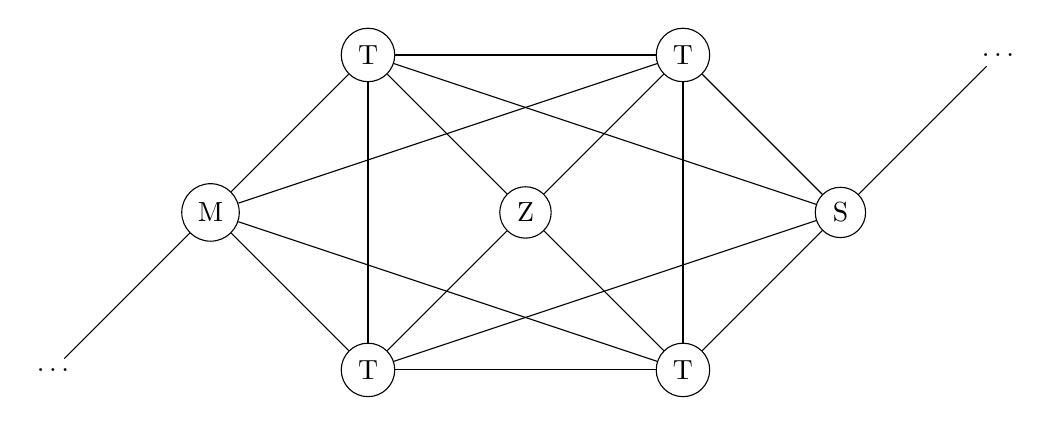
\begin{tikzpicture}[node distance = 2cm]
	\tikzset{VertexStyle/.style = {
			shape=circle,
			draw=black
	}}
	\node[VertexStyle] (1) {Z};
	\node[VertexStyle, left of=1, above of=1] (2) {T};
	\node[VertexStyle, right of=1, above of=1] (3) {T};
	\node[VertexStyle, left of=1, below of=1] (4) {T};
	\node[VertexStyle, right of=1, below of=1] (5) {T};
	\node[VertexStyle, left of=2, below of=2] (6) {M};
	\node[VertexStyle, right of=5, above of=5] (7) {S};
	\node[right of=7, above of=7] (8) {$\dots$};
	\node[left of=6, below of=6] (9) {$\dots$};
	
	\path [-] (1) edge node[left] {} (2);
	\path [-] (1) edge node[left] {} (3);
	\path [-] (1) edge node[left] {} (4);
	\path [-] (1) edge node[left] {} (5);
	\path [-] (3) edge node[left] {} (2);
	\path [-] (4) edge node[left] {} (2);
	\path [-] (5) edge node[left] {} (3);
	\path [-] (5) edge node[left] {} (4);
	\path [-] (2) edge node[left] {} (6);
	\path [-] (3) edge node[left] {} (6);
	\path [-] (4) edge node[left] {} (6);
	\path [-] (5) edge node[left] {} (6);
	\path [-] (2) edge node[left] {} (7);
	\path [-] (3) edge node[left] {} (7);
	\path [-] (4) edge node[left] {} (7);
	\path [-] (5) edge node[left] {} (7);
	\path [-] (7) edge node[left] {} (8);
	\path [-] (6) edge node[left] {} (9);
	\end{tikzpicture}
	\caption[Example slice]{Example slice}
	\label{fig:example_slice}
\end{figure}

\subsection{Using background knowledge during model construction}
In the case of production facilities, the basic structure of the facility itself, even more so in a modularized system like the one on hand, has to be integrated into the basic graph scheme. Considering inherent parallelisms in the system (like two modules working in parallel), already places a few constraints on the resulting input graphs. Constraints were mostly input manually into the system prior to graph construction.

\section{Features of interest}
As mentioned before, the production facility doesn't run at peak performance most of the time. As such, of interest to this analysis was mostly if specific events or sequence of events would be able to predict a decrease in the OOE figure. A sequence analysis performed by my advisor some time before this thesis had already yielded some preliminary results in this direction which were considered known problems by the experts. Stumbling upon a pattern which would be considered a novel mechanical problem to solve would be the prime result of this work.

\section{Modified gSpan}
\label{section:gspan}
\textit{gSpan} was first introduced by Yan and Han in 2002.\cite{Yan2002-sj}\cite{Yan2002-hg} \textit{gSpan} leverages depth-first search (DFS) to map graphs to minimum DFS codes, which are a canonical lexicographic graph labeling method. As all isomorphic graphs have the same canonical label, once computation of the labels is completed, it's trivially easy to solve the isomorphism question for any two graphs by comparing their canonical labels. If those labels are available in a lexicographic format, their comparison in itself is also trivially achievable by simple string comparison. The modification of \textit{gSpan} in this work is based on adding a hash function to make the lexicographic comparison faster.

Introducing a hashing algorithm obviously introduces the risk of collisions between hashes, rendering the formerly unambiguous canonical label to graph mapping no longer bijective, but instead surjective. In the case of structured or semi-structured operator controlled inputs, however, the theoretical possibility of collisions because of the hashing shouldn't be a huge concern.


\subsection{DFS Lexicographic Order}
To demonstrate the construction of a minimum DFS code, we're again using the example graph from chapter \ref{chapter:theoretical_basis}, this time with additional labels for nodes and edges as visualized in figure \ref{fig:example_graph_dfs}.
\begin{figure}
	\centering
	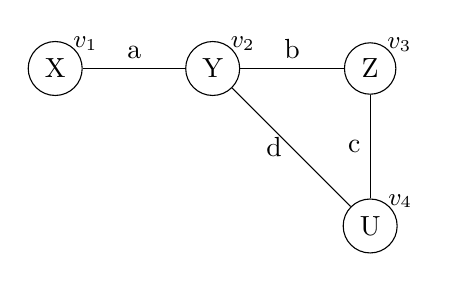
\begin{tikzpicture}[node distance = 2cm]
	\tikzset{VertexStyle/.style = {
		shape=circle,
		draw=black
	}}
	\node[VertexStyle, label={[label distance=-.2cm]45:\small $v_1$}] (1){X};
	\node[VertexStyle, right of= 1, label={[label distance=-.2cm]45:\small $v_2$}] (2){Y};	
	\node[VertexStyle, right of= 2, label={[label distance=-.2cm]45:\small $v_3$}] (3){Z};
	\node[VertexStyle, below of= 2, right of=2, label={[label distance=-.2cm]45:\small $v_4$}] (4){U};
	
	\path [-] (1) edge node[above] {a} (2);
	\path [-] (2) edge node[above] {b} (3);
	\path [-] (3) edge node[left] {c} (4);
	\path [-] (2) edge node[left] {d} (4);
	\end{tikzpicture}
	\caption[Graph $G$ from chapter \ref{chapter:theoretical_basis} with labels]{Graph $G$ from chapter \ref{chapter:theoretical_basis} with labels}
	\label{fig:example_graph_dfs}
\end{figure}

Mapping this graph to a minimum DFS code using algorithm \ref{alg:mindfscode} yields the minimum DFS code in table \ref{table:dummy_min_dfs_codes}.
\begin{table}[h]
	\centering
	\caption{Minimum DFS code of graph $G$}
	\label{table:dummy_min_dfs_codes}
	\begin{tabular}{l|l}
		edge no. & DFS code          \\ \hline
		0        & $(0,2,U,d,Y)$     \\
		1        & $(1, 2, X, a, Y)$ \\
		2        & $(0, 3, U, c,Z)$  \\
		3        & $(2, 3, Y, b, Z)$
	\end{tabular}
\end{table}

\begin{algorithm}
	\caption{MinDFSCode($G$)}\label{alg:mindfscode}
	\begin{algorithmic}[1]
		\State {initiate $S \gets \emptyset$}
		\ForEach {vertex $v \in V(G)$}
		\State {perform a depth-first search with $v$ as a starting point;}
		\State {transform the resulting DFS tree $t$ into a DFS code tuple;}
		\EndFor
		\State {sort DFS code tuples by comparing their length according to DFS lexicographic order and choose the smallest one as the canonical label}
	\end{algorithmic}
\end{algorithm}
The DFS lexicographic order is a linear order defined by the less or equal function in algorithm \ref{alg:dfs_lexicographic_order}. For the neighborhood restrictions and the comparison function between two DFS code tuples $a = (i_a, j_a, l_{i_a}, l_{(i_a, j_a)}, l_{j_a})$ and $b = (i_b, j_b, l_{i_b}, l_{(i_b, j_b)}, l_{j_b})$, please see algorithm \ref{alg:dfs_lexicographic_order_tuples}. In both algorithms, the following definitions apply: $\alpha = (a_0, a_1, ..., a_m)$ and $\beta = (b_0, b_1, ..., b_n)$, where each $a_t, b_t$ is a DFS code tuple of the form $x_t = (i_x, j_x, l_{i_x}, l_{(i_x, j_x)}, l_{j_x})$. $i_x, j_x$ are vertices, $l_{i_x}, l_{j_x}$ are their labels, and $l_{(i_x, j_x)}$ is the edge label.

\begin{algorithm}
	\caption{DFSLexicographicLE($\alpha, \beta$)}\label{alg:dfs_lexicographic_order}
	\begin{algorithmic}[1]
		\If {$n \geq m$ and $a_m = b_m$}
			\State\Return {True, ie $\alpha \leq \beta$}
		\Else
			\State {$a_{\text{forward}} \gets \text{Bool}(j_a > i_a)$}
			\State {$b_{\text{forward}} \gets \text{Bool}(j_b > i_b)$}
			\State {$a_{\text{backward}} = \neg a_{\text{forward}}$}
			\State {$b_{\text{backward}} = \neg b_{\text{forward}}$}
			\If{$a_{\text{forward}} \land b_{\text{forward}}$}
				\State\Return {True, ie $\alpha \leq \beta$}
			\EndIf
			\If{$a_{\text{backward}} \land b_{\text{backward}} \land j_a < j_b$}
				\State\Return {True, ie $\alpha \leq \beta$}
			\EndIf
			\If{$a_{\text{backward}} \land b_{\text{backward}} \land j_a = j_b \land l_{(i_a, j_a)} < l_{(i_b, j_b)}$}
				\State\Return {True, ie $\alpha \leq \beta$}
			\EndIf
			\If{$a_{\text{forward}} \land b_{\text{forward}} \land i_b < i_a$}
				\State\Return {True, ie $\alpha \leq \beta$}
			\EndIf
			\If{$a_{\text{forward}} \land b_{\text{forward}} \land i_b = i_a \land l_{i_a} < l_{i_b}$}
				\State\Return {True, ie $\alpha \leq \beta$}
			\EndIf
			\If{$a_{\text{forward}} \land b_{\text{forward}} \land i_b = i_a \land l_{i_a} = l_{i_b} \land l_{(i_a, j_a)} < l_{(i_b, j_b)}$}
				\State\Return {True, ie $\alpha \leq \beta$}
			\EndIf
			\If{$a_{\text{forward}} \land b_{\text{forward}} \land i_b = i_a \land l_{i_a} = l_{i_b} \land l_{(i_a, j_a)} = l_{(i_b, j_b)} \land l_{j_a} < l_{j_b}$}
				\State\Return {True, ie $\alpha \leq \beta$}
			\EndIf
			\State\Return {False, ie $\alpha > \beta$}
		\EndIf
	\end{algorithmic}
\end{algorithm}

\begin{algorithm}
	\caption{DFSTuplesLexicographicLE($a, b$)}\label{alg:dfs_lexicographic_order_tuples}
	\begin{algorithmic}[1]
		\State {$a_{\text{forward}} \gets \text{Bool}(j_a > i_a)$}
		\State {$b_{\text{forward}} \gets \text{Bool}(j_b > i_b)$}
		\State {$a_{\text{backward}} = \neg a_{\text{forward}}$}
		\State {$b_{\text{backward}} = \neg b_{\text{forward}}$}
		\If{$a_{\text{forward}} \land b_{\text{forward}} \land a_j < b_j$}
			\State\Return {True, ie $a \leq b$}
		\EndIf
		\If{$a_{\text{backward}} \land b_{\text{backward}} \land (a_i < b_i \lor (a_i = b_i \land a_j < b_j))$}
			\State\Return {True, ie $a \leq b$}
		\EndIf
		\If{$a_{\text{backward}} \land b_{\text{forward}} \land a_i < b_j$}
			\State\Return {True, ie $a \leq b$}
		\EndIf
		\If{$a_{\text{forward}} \land b_{\text{backward}} \land b_j \leq a_i$}
			\State\Return {True, ie $a \leq b$}
		\EndIf
		\If{$a_{\text{backward}}$}
			\If{$b_{\text{forward}} \land b_i \leq a_i \land b_j = a_i + 1$}
				\State\Return {True, ie $a \leq b$}
			\EndIf
			\If{$b_{\text{backward}} \land b_i = a_i \land a_j < b_j$}
				\State\Return {True, ie $a \leq b$}
			\EndIf
		\EndIf
		\If{$a_{\text{forward}}$}
			\If{$b_{\text{forward}} \land b_i \leq a_j \land b_j = a_j + 1$}
				\State\Return {True, ie $a \leq b$}
			\EndIf
			\If{$b_{\text{backward}} \land b_i = a_j \land b_j < a_i$}
				\State\Return {True, ie $a \leq b$}
			\EndIf
		\EndIf
		\State\Return {False, ie $a > b$}
		
	\end{algorithmic}
\end{algorithm}

With these comparison algorithms in place, a \textit{DFS Code Tree} can be constructed. In a \textit{DFS Code Tree}, each node represents one graph via its DFS code. Obviously, in such a tree, the DFS code for a graph can turn up more than once, depending on node addition order. Thus, the first code that turns up on a pre-order depth-first search of the \textit{DFS Code Tree} is what we previously called the minimum DFS code.

This results in the more formal definition given by \cite{Yan2002-hg}:
\begin{quotation}
	Given a graph $G$, $Z(G) = \{code(G, T) | \forall T, T \text{ is a DFS code}\}$, based on DFS lexicographic order, the minimum one, $\min(Z(G))$, is called \textbf{Minimum DFS Code} of $G$. It is also the canonical label of $G$.
\end{quotation}

\subsection{Graphset projection and subgraph mining}
The pattern growth approach now becomes clearer when we're trying to construct a new pattern from an already found one: to construct a valid DFS code for the new pattern, the new edge cannot be added at an arbitrary position, but can only be added to vertices on the ''rightmost path.`` This is further limited, as only forward edges can grow from all vertices on the rightmost path, whereas backward edges can only be grown from the rightmost vertex.

With these definitions in place, the \textit{gSpan} algorithm works as follows (see algorithm \ref{alg:graph_set_projection} for the pseudocode):

\begin{algorithm}
	\caption[GraphSet\_Projection($\mathcal{D,S}$)]{GraphSet\_Projection($\mathcal{D,S}$)\cite{Yan2002-hg}}
	\label{alg:graph_set_projection}
	\begin{algorithmic}[1]
		\State sort labels of the vertices and edges in $\mathcal D$ by their frequency;
		\State remove infrequent vertices and edges;
		\State relabel the remaining vertices and edges in descending frequency;
		\State $\mathcal S^1 \gets \text{all frequent 1-edge graphs in } \mathcal D$;
		\State sort $\mathcal S^1$ in DFS lexicographic order;
		\State $\mathcal S \gets \mathcal S^1$;
		\ForEach {$\text{edge }e \in \mathcal S^1$}
		\State $\text{initialize } s \text{with } e, \text{set } s.GS = \{g | \forall g \in \mathcal D, e \in E(g)\}$;
		\State Subgraph\_Mining($\mathcal{D, S}, s$);
		\State $\mathcal D \gets \mathcal D - e$;
		\If {$|\mathcal D| < \textit{min\_sup}$}
		\State \textbf{break};
		\EndIf
		\EndFor
	\end{algorithmic}
\end{algorithm}

In a first step, infrequent single nodes and edges are removed from the search space, as there can be no longer patterns with infrequent substructures in them. The frequent one-edge subgraphs are stored in $\mathcal S^1$ and will be used as the seeds from which longer patterns are grown by calling algorithm \ref{alg:subgraph_mining} on all such one-edge patterns. Along the way, the graph set $\mathcal{D}$ is consecutively shrunk during each iteration, as previously searched patterns cannot turn up again later on. After finding all one-edge patterns and all their decedents, the algorithm terminates. For a definition of Enumerate(), see \cite{Yan2002-hg}.

\begin{algorithm}
	\caption[Subgraph\_Mining($\mathcal{D, S}, s$)]{Subgraph\_Mining($\mathcal{D, S}, s$)\cite{Yan2002-hg}}
	\label{alg:subgraph_mining}
	\begin{algorithmic}[1]
		\If {$\textit{s} \neq \textit{min}(s)$}
		\State \textbf{return};
		\EndIf
		\State $\mathcal S \gets \mathcal S \cup \{s\}$
		\State generate all \textit{s'} potential children with one edge growth;
		\State Enumerate(\textit{s});
		\ForEach {$c, c \text{ is } s' \text{ child}$}
		\If {$\textit{support}(c) \geq \textit{min\_sup}$}
		\State $s \gets c;$
		\State Subgraph\_Mining($\mathcal{D, S}, s$);
		\EndIf
		\EndFor
	\end{algorithmic}
\end{algorithm}

\section{Support Vector Machine}
An SVM\cite{Cortes1995-ix} is a supervised machine learning model that can classify a data set into distinct groups by constructing a hyperplane between their feature vectors that maximizes the distance between the nearest data points and the hyperplane for any class (the functional margin). Figure \ref{fig:hyperplane} illustrates this for a simple, two dimensional example with two intuitively distinct classes. The samples on the margin are called the support vectors. The SVM module from the Python package scikit-learn\cite{Pedregosa2011-ld} was used.
\begin{figure}
	\centering
	\noindent\includegraphics[width=\linewidth]{images/sphx_glr_plot_separating_hyperplane_0011}
	\caption[Functional margin between two classes of data points]{Functional margin between two classes of data points\cite{noauthor_undated-io}}
	\label{fig:hyperplane}
\end{figure}

The original problem formulation for support vector classification is as follows:\cite{Chang2011-wa}

Let $\boldsymbol{x}_i \in \mathbb{R}^p$ with $i=1,...,n$ and let $\boldsymbol{y} \in \mathbb{R}^l$ be an indicator vector, such that $\boldsymbol{y}_i \in \{1, -1\}$. Then SVC solves the following primal optimization problem:
\[\min_ {w, b, \zeta} \frac{1}{2} w^T w + C \sum_{i=1}^{n} \zeta_i \]
subject to
\[ y_i (w^T \phi (x_i) + b) \geq 1 - \zeta_i,
\zeta_i \geq 0, i=1, ..., n\]
with its dual being
\[\min_{\alpha} \frac{1}{2} \alpha^T Q \alpha - e^T \alpha\]
subject to
\[y^T \alpha = 0,
0 \leq \alpha_i \leq C, i=1, ..., n\]
where $\phi(\boldsymbol{x}_i)$ maps $\boldsymbol{x}_i$ into a higher-dimensional space, $e$ is the vector of all ones, $Q$ is an $x \times x$ positive semidefinite matrix with $Q_{ij} = y_i y_j K(x_i, x_j)$, with $K(x_i, x_j) = \phi(x_i)^T\phi(x_j)$ being the kernel, and $C > 0$ is the regularization parameter (upper bound).
The decision function is given by:
\[\operatorname{sgn}\left(\sum_{i=1}^n y_i \alpha_i K(x_i, x) + \rho\right).\]

\section{OEE anomaly detection}
Site performance is measured through OEE (Overall Equipment Effectiveness) scoring. OEE calculation yields a scoring between 0 and 1 according to the following formula:
\[OEE = \frac{POK \cdot CT}{OT},\]
where \textit{POK} is the number of \textbf{p}arts that came out of quality control \textbf{OK}, \textit{CT} is the \textbf{c}ycle \textbf{t}ime in seconds per part and \textit{OT} is the \textbf{o}perational \textbf{t}ime of the assembly line in seconds. All values are reset during shift changes, resulting in a short period of 0\% OEE before the first part of a new shift is produced. As an example, if the line ran for 3600 seconds, needed 10 seconds to produce a part and produced 300, the resulting OEE score would be
\[OEE = \frac{300 \cdot 10}{3600}\approx .83. \]
This result would indicate an assembly line running with about 83\% effectiveness. It should've produced 60 parts more in the given time, and, thus, was held up for some reason or another about 17\% of the time.

OEE scores were available as a time series for the same time frame as the factory data set. As OEE scores were calculated every second, the resulting data set was considerably larger than the error logs, consisting of more than 800,000 rows of 26 columns, most of which weren't used. Anomaly detection consisted mainly of identifying more or less sudden drops in OEE scoring, indicating times when no parts were produced. The first few anomaly detection systems proved very capable of detecting shift changes and not much else, while later iterations did indeed pick up on most of the intuitively obvious drops.

Algorithm \ref{alg:oeedetectanomalies} provides an efficient anomaly detection algorithm with $O(n)$ complexity, with $S$ being a set of slope indicators, $\tilde{S}$ the mean slope indication and $c$ a manually set parameter for how many standard deviations from the mean slope a anomaly should be assumed.

\begin{algorithm}
	\caption{OEEDetectAnomalies(OEE\_data)}\label{alg:oeedetectanomalies}
	\begin{algorithmic}[1]
		\State {$S \gets \emptyset$;}
		\State {$R \gets \emptyset$;}
		\ForEach {5 minute slice $\boldsymbol{s}$;}
		\If {$\min_{OEE} \boldsymbol{s} \neq 0$;}
		\State {$x \gets \frac{\max_{t} \boldsymbol{s}}{\min_{t} \boldsymbol{s}} -1 $;}
		\State {$S \gets S \cup x$;}
		\Else
		\State {$S \gets S \cup 0$;}
		\EndIf
		\EndFor
		\State {$l \gets \tilde{S} - c \cdot SD(S)$;}
		\ForEach {$\hat{\boldsymbol{s}} = (x, y, z)$ in $S, z<l$;}
		\State {$R \gets R \cup \hat{\boldsymbol{s}}$;}
		\EndFor \\
		\Return {$R$;}
	\end{algorithmic}
\end{algorithm}
\chapter{Experiments and performance study}
\section{Test setup}
All tests were performed on a 2015 Lenovo Thinkpad T450s, with 12GB of RAM and an Intel Core i7-5600U clocked at 2.6 GHz, running a NixOS 17.09 with Python 3.6.4 built with GCC 6.4.0.
\section{Results for a synthetic data set}
\label{section:synthetic_data_results}
The synthetic data set was generated by first simulating a random walk of OEE values from 11 am until about 9 pm, mimicking about one shift (figure \ref{fig:dummyrandomwalk}). Later, equivalent error logs were created, with some messages more likely to turn up at times when the generated random walk resulted in an OEE drop as recognized by the OEE anomalies detection.

\begin{figure}
	\centering
	\includegraphics[width=1\linewidth]{images/dummy_random_walk}
	\caption{Synthetic OEE values}
	\label{fig:dummyrandomwalk}
\end{figure}

These generated data look similar to the real facility set, with various drops and and ascents. Resulting patterns like figure \ref{fig:dumm_pattern} also look very similar to real patterns like figure \ref{fig:small_pattern} above.

\begin{figure}
	\centering
	\includegraphics[width=1\linewidth]{images/dummy_pattern}
	\caption{8-edge pattern from the synthetic data set, min\_sup = .4}
	\label{fig:dumm_pattern}
\end{figure}

The synthetic error log consisted of 1000 rows of errors, the OEE set of 35,919 rows (roughly 9 hours of second by second logs). Run times were very manageable for higher min\_sup values, but soon reached exponential (and thus, unsustainable) growth for min\_sup values much lower than .2 (cf. table \ref{table:runtimes_syn}).

\begin{table}[]
	\centering
	\caption{Run times and patterns found (synthetic data set)}
	\label{table:runtimes_syn}
	\begin{tabular}{l|l|l}
		data set                                      & \textit{t} & patterns \\ \hline
		import errors and graph generation            & 1s         &          \\
		import and anomalies detection on OEE         & 8s         &          \\ \hline
		\textit{gSpan} (min\_sup = .7)                & 2s         & 40       \\
		\textit{gSpan} (min\_sup = .6)                & 8s         & 106      \\
		\textit{gSpan} (min\_sup = .5)                & 19s        & 241      \\
		\textit{gSpan} (min\_sup = .4)                & 74s        & 1056     \\ \hline
		SVM training and validation   (min\_sup = .7) & 4s         &          \\
		SVM training and validation   (min\_sup = .6) & 8s         &          \\
		SVM training and validation   (min\_sup = .5) & 35s        &          \\
		SVM training and validation   (min\_sup = .4) & 13m 14s    &
	\end{tabular}
\end{table}

\subsection{Evaluation with OEE data set}
OEE anomalies were split into a training data set and an validation data set, with 80\% of the data being used for training and the remaining 20\% used for validation. For the min\_sup = .5 run, experimental mean slope $\tilde{S}$ (cf. algorithm \ref{alg:oeedetectanomalies}) was .5 with a standard deviation of .21 and a $c$-value of .1. The validation data set consisted of 49 time windows, 33 of which were deemed as a noticeable drop by the OEE evaluation algorithm. Of these 33, the SVM correctly identified 28 as drops, for a sensitivity score of 85\%. Of the remaining 19 non-drops, 5 were falsely identified as positives, for a specificity score of 74\%.

For the min\_sup = .4 run, experimental mean slope $\tilde{S}$ was .5 with a standard deviation of .21 and a $c$-value of .1. The validation data set consisted of 49 time windows, 33 of which were deemed as a noticeable drop by the OEE evaluation algorithm. Of these 33, the SVM correctly identified 28 as drops, for a sensitivity score of 84.85\%. Of the remaining 19 non-drops, 5 were falsely identified as positives, for a specificity score of 73.68\%.
\section{Results for facility data set}
The facility data set consisted of 57,171 rows of error logs and 802,800 rows of OEE evaluation data. Results with min\_sup values of less than .5 could not be achieved. The algorithm consistently used up so much memory that it was OOM killed by the operating system after about a day of run time.

\begin{table}
	\centering
	\caption{Run times and patterns found (facility data set)}
	\label{table:runtimes_real} 
	\begin{tabular}{l|l|l}
		data set                                      & \textit{t}          & patterns \\ \hline
		import errors and graph generation            & 50s                 &          \\
		import and anomalies detection on OEE         & 2m 27s              &          \\ \hline
		\textit{gSpan} (min\_sup = .9)                & 2m 20s              & 12       \\
		\textit{gSpan} (min\_sup = .7)                & 6h 27m 12s          & 846      \\
		\textit{gSpan} (min\_sup = .5)                & \textit{OOM killed} & --       \\ \hline
		SVM training and validation   (min\_sup = .7) & 27s                 &
	\end{tabular}
\end{table}

\subsection{Evaluation with OEE data set}
\label{subsection:evaluation}
OEE anomalies were split as above. Experimental mean slope $\tilde{S}$ (cf. algorithm \ref{alg:oeedetectanomalies}) was 1.1 with a standard deviation of .16 and a $c$-value of .1. The validation data set consisted of 486 time windows, 64 of which were deemed as a noticeable drop by the OEE evaluation algorithm. Of these 64, the SVM trained on patterns with a min\_sup of .7 correctly identified 60 as drops, for a sensitivity score of 93.75\%. Of the remaining 422 non-drops, 18 were identified as false positives, for a specificity score of 95.73\%.

\chapter{Summary and Discussion}
To conclude this bachelor's thesis, the following will summarize my findings with the acknowledgment that, although the essential research in this work was of my own design and execution, a project such as this is virtually impossible without guidance by an advisor and support by friends and family.

With this work, I've introduced a method and provided a Python program to mine error log data for useful patterns, using a graph representation to take advantage of structural information and incorporate outside expert knowledge. I touched upon the most important concepts on which my model assumptions rest and expounded on some approaches that did not yield usable results.

The proposed algorithm has been shown to produce patterns with adequate experimental time complexity, with synthetic data and proprietary Siemens facility data. The found patterns, to a first approximation, seem to provide real informational value and seem able to predict facility downtimes, as measured by a drop in OEE, all to a reasonable degree. A possible next step would be to show the patterns and the thoughts that went into the OEE anomaly detection to an expert with domain knowledge and then refine the proposed approaches through a few more iterations.

The proposed approach has been shown to be somewhat fragile, in that at least some implementation details of \textit{gSpan}, the overall data structure used in this work, and maybe even the included libraries should be reevaluated at a later time, to hammer out possible errors and improve on the interaction between parts. 

Further improvements to the algorithm, especially to improve on average-case time and memory performance, and allow it to directly process data streams instead of stale data would be much appreciated, but are sadly out of scope for this bachelor's thesis.

The results that \textit{could} be reached, however, point in a promising direction. The overall approach -- leveraging a graph-based mining algorithm against a time series of event logs -- seems to have merit, not least of all because the resulting patterns can be visualized in a way that immediately makes a lot of sense to both the casual observer as well as the expert with intimate domain knowledge.

This remains true even if event logs don't immediately spring to mind as being structurally similar to networks and as such means this approach needs further research and should at least be tried again with similarly non-obvious graph data in the future.

\chapter*{Acknowledgments}
\addcontentsline{toc}{chapter}{Acknowledgements}  
I want to thank first and foremost my advisor, Martin Ringsquandl, as without his ever intelligent and on-point criticisms and ideas this bachelor's thesis wouldn't have been possible. Second, Prof. Dr. Kröger, for allowing this thesis as an external bachelor's thesis at the Munich Siemens AG headquarters. Third, Siemens Corporate Technology, and all the intelligent and lovely folks at the Research, Development and Automation/Business Analytics and Monitoring unit, who provided valuable input not only during lunch hours. I also wish to thank all my friends and family, who constantly bugged me about my progress especially during the later stages, especially Irina, Christina and my mother. Last, but certainly not least, I also want to thank my cat Tigris, who bugged me as well while I was writing, although he was mostly out for food.

\sloppy{Furthermore, I am very thankful to live in a time with tools such as  \mbox{CytoScape}\cite{Shannon2003-gg},\mbox{TeXStudio}\cite{Van_der_Zander_undated-kf}, \mbox{TeXLive}\cite{Rahtz_undated-bv}, \mbox{IntelliJ PyCharm}, and \mbox{PaperPile} for making the development of my analytics software and the later write-up much easier and more efficient.}

\listoffigures
\listoftables
\listof{algorithm}{List of Algorithms}
\bibliographystyle{utcaps}
\bibliography{bibliography}

\end{document}
